\section{Data and theory}
\label{sec:theory}

In this work, the photon content of the proton $x\gamma(x,Q^2)$ is
extracted from a PDF analysis based on the combined inclusive DIS
cross-section data from HERA~\cite{Abramowicz:2015mha}
supplemented by the ATLAS measurements of high-mass Drell-Yan
differential cross sections at $\sqrt{s}=8$ TeV~\cite{Aad:2016zzw}.
%
The HERA inclusive data are the backbone of modern PDF fits, providing
information on the quark and gluon content of the proton, while
the high-mass Drell-Yan data provide a direct sensitivity to the
photon PDF.
%
As illustrated in Fig.~\ref{fig:photoninduced}, 
 dilepton production at hadron colliders can arise
from either quark-antiquark $s$-channel scattering, or from
photon-photon $t$- and $u$-channel scattering mediated by a lepton.

The ATLAS high-mass Drell-Yan 8 TeV measurements are presented in terms
of both the
single-differential (1D) invariant-mass distribution,
$d\sigma/dm_{ll}$, as well as double-differential (2D)
distributions in $m_{ll}$ and $y_{ll}$, namely
$d^{2}\sigma/dm_{ll}d|y_{ll}|$, and in $m_{ll}$ and $\Delta\eta_{ll}$,
$d^{2}\sigma/dm_{ll}\Delta\eta_{ll}$.
%, where $m_{ll}$, $y_{ll}$ and $\Delta\eta_{ll}$
%denote the invariant mass, rapidity, and separation in pseudo-rapidity
%of the lepton pair, respectively.
%
For the invariant-mass 1D distribution, there are 12 bins between $m_{ll}=116$ GeV
and 1.5 TeV; and for both double-differential distributions,
there are five different bins in invariant mass,
from the lowest bin with 116 GeV < $m_{ll}$ <
150 GeV to the highest bin with 500 GeV < $m_{ll}$ < 1500 GeV.
 %
The first three (last two) $m_{ll}$ bins of the 2D distributions are divided into 12 (6) bins
with fixed width, extending up to 2.4 and 3.0 for the $|y_{ll}|$
and $|\Delta\eta_{ll}|$ distributions, respectively.
%

The photons which undergo hard scattering in the
$\gamma\gamma \to ee$  process from Fig.~\ref{fig:photoninduced}
can be produced by either  emission from the
proton as a whole (the ``elastic'' component) or radiated by the constituent quarks
(the ``inelastic'' component).
%
%In the ATLAS high-mass DY measurement, the double elastic component is suppressed
% by the
% requirement of having more than two primary tracks~\cite{Aad:2016zzw}.
% %
% Moreover, the inelastic-elastic photon scattering corresponds to only about
% 10\% of the total measured cross sections.
% %
 From the theory point of view, the photon PDF extracted from the
 fit is by construction the sum of the elastic and inelastic contributions,
 though this analysis is mostly sensitive to the latter.

For the calculation of NLO high-mass Drell-Yan cross sections, the
{\tt MadGraph5{\_}aMC@\-NLO}~\cite{Alwall:2014hca} program is used, which
includes the contribution from photon-initiated diagrams, interfaced
to {\tt APPLgrid}~\cite{Carli:2010rw} through {\tt
  aMCfast}~\cite{amcfast}.
%
A tailored version of {\tt APPLgrid} is used, accounting for
the contribution of the photon-initiated processes \footnote{Modified version of {\tt APPLgrid} available at: {\tt https://github.com/scarrazza/applgridphoton}}.
%
The calculation is performed in the $n_f=5$ scheme neglecting mass
effects of charm and bottom quarks in the matrix elements, as
appropriate for a high-scale process.
%
These NLO theoretical predictions match the  
analysis cuts of the data, with $m_{ll}\ge 116$ GeV, $\eta_l\le 2.5$, and
$p_T^l \ge 40$ GeV$~(30)$ GeV for the leading (sub-leading) lepton being
the most important ones.
%
As discussed below, the NLO calculations are then supplemented by
NNLO/NLO $K$-factors obtained from {\tt FEWZ}~\cite{Gavin:2012sy}.
%
The NLO EW corrections to the DY processes are also estimated
using {\tt FEWZ}. 
%
The photon-initiated process is taken at LO since this corresponds to
the {\tt APPLgrid} implementation and the NLO corrections are
very small compared to the data accuracy.
%

%%%%%%%%%%%%%%%%%%%%%%%%%%%%%%%%%%%%%%%%%%%%%%%%%%%%%%%%%%%%%%%%
\begin{figure}[t]
  \begin{center}
    \includegraphics[width=0.95\columnwidth]{figs/DYdiagrams.pdf}
    \end{center}
    \caption{Diagrams that contribute to lepton-pair production at
      hadron colliders at the Born level.}
\label{fig:photoninduced}
\end{figure}
%%%%%%%%%%%%%%%%%%%%%%%%%%%%%%%%%%%%%%%%%%%%%%%%%%%%%%%%%%%%%%%%

The DIS structure functions and PDF evolution are computed with the {\tt
  APFEL} program~\cite{Bertone:2013vaa}, which is currently accurate
up to NNLO in QCD and NLO in QED, including the relevant mixed
QCD+QED corrections.
%
This means that, on top of the pure QCD
contributions, the DGLAP evolution
equations~\cite{Gribov:1972ri,Dokshitzer:1977,Altarelli:1977zs} are
solved including the $\mathcal{O}\lp \alpha_s\alpha\rp$ and
$\mathcal{O}\lp \alpha^2\rp$ corrections to the splitting functions.
%
%Concerning the DIS structure functions, 
Corrections of $\mathcal{O}\lp \alpha\rp$ are also included leading to a (weak)
explicit dependence of the predictions on the photon PDF.
%
Details
of the implementation of these corrections and of their numerical
impact are given in Appendix~\ref{sec:appendixAPFEL}.
%
Heavy-quark (charm and bottom) mass effects to DIS structure functions
are taken into account using the FONLL-B~(C) general-mass
scheme~\cite{Forte:2010ta} for the NLO~(NNLO) fits.
%
The numerical values of the heavy-quark masses in the mass parameter 
scheme
are taken to be $m_c=1.47~$GeV and $m_b=4.5~$GeV as determined in~\cite{Abramowicz:2015mha},  
consistent with the latest PDG averages~\cite{Agashe:2014kda}.
%
The reference values of the QCD and QED coupling constants are chosen to be
$\alpha_s(m_Z)=0.118$ and $\alpha(m_\tau=1.777\mbox{ GeV})=1/133.4$, again consistent
with the PDG recommended values.

In the  calculation of the Drell-Yan cross section, the
dynamical renormalisation $\mu_{R}$ and factorisation $\mu_{F}$
scales are used, which are set equal to the scale of invariant mass $m_{ll}$,
both for the quark- and gluon-induced and for the photon-induced
contributions.
%
The choice of other values for these scales in the QED diagrams,
such as a fixed scale $\mu_R=\mu_F=M_Z$, leads 
to  variations of the photon-initiated cross-sections of at most a few percent.
%
The choice of the scale for the photon PDF  is further discussed
in~\cite{Harland-Lang:2016lhw,Dittmaier:2009cr}.
%
For the kinematics of the ATLAS DY data, the ratio between the photon-initiated
contributions and  quark- and gluon-induced dilepton production is largest
for central rapidities and large invariant masses. 
%
For the most central (forward) rapidity
bin, $0 < |y_{ll}| < 0.2$ ($2.0 < |y_{ll}| < 2.4$), the ratio
between the QED and QCD contributions varies between 2.5\%~(2\%) at low
invariant masses and 12\%~(2.5\%) for the highest $m_{ll}$ bin.
%
Therefore, data from the central region will exhibit the highest
sensitivity to $x\gamma(x,Q^2)$.

The {\tt MadGraph5{\_}aMC@NLO} NLO QCD and LO QED calculations used in this work have been
benchmarked against the corresponding predictions  obtained with the {\tt FEWZ}
code~\cite{Gavin:2012sy}, finding agreement within statistical uncertainties of
the predictions for both the 1D and the 2D distributions.

%
In order to achieve NNLO QCD and NLO EW accuracy in our theoretical
calculations, the NLO QCD and LO QED cross-sections computed with
{\tt MadGraph5{\_}aMC@NLO}
have been supplemented by bin-by-bin $K$-factors
defined as:
\begin{equation}
  \label{eq:kfactor}
  K(m_{ll},|y_{ll}|) \equiv\frac{\rm NNLO\  QCD  + NLO\  EW}{\rm NLO\  QCD + LO\  EW} \, ,
\end{equation}
using the MMHT2014 NNLO~\cite{Harland-Lang:2014zoa} PDF set both in
the numerator and in the denominator. 
%
The $K$-factors have been computed using
   {\tt FEWZ}  with the same settings and analysis cuts as the corresponding
   NLO calculations of {\tt MadGraph5{\_}aMC@NLO}.
%
This approximation is justified since NNLO $K$-factors depend very
mildly on the input PDF set, see for example~\cite{Czakon:2016olj}.
%
The photon induced contribution, as provided in \cite{Aad:2016zzw},  has been explicitly 
subtracted from the {\tt FEWZ} predictions.
 %
   Fig.~\ref{fig:kf} shows the $K$-factors of  Eq.~({\ref{eq:kfactor})
  corresponding to the double differential $(m_{ll},|y_{ll}|)$
  cross sections 
  as a function of the dilepton
  rapidity $|y_{ll}|$, where each set of points corresponds to a different
  dilepton invariant mass $m_{ll}$ bin.
%
  The $K$-factors vary between 0.98 and 1.04,
  highlighting the fact that higher-order corrections to the Drell-Yan
  process are moderate, in particular at low values of $m_{ll}$ and in
  the central region.
%
  Even at forward rapidities, the $K$-factors modify the NLO result by
  at most 4\%.

  %%%%%%%%%%%%%%%%%%%%%%%%%%%%%%%%%%%%%%%%%%%%%%%%%%%%%%%%
\begin{figure}[t]
\centering
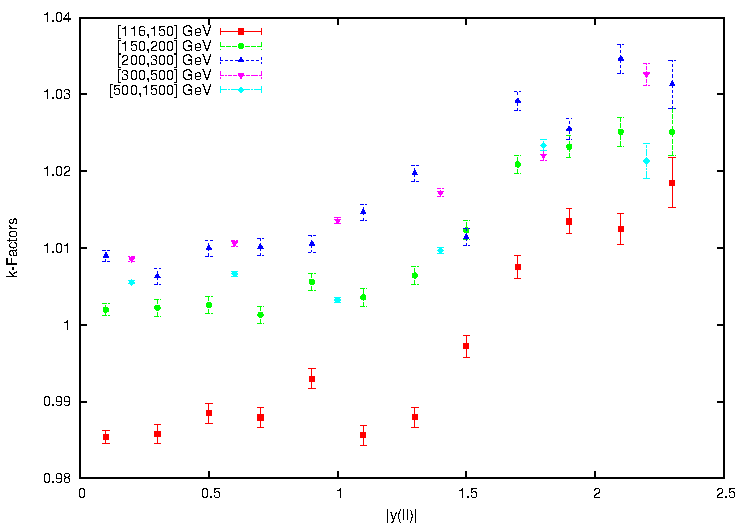
\includegraphics[width=0.95\columnwidth]{figs/kF_2D.pdf}
\caption{The NNLO/NLO $K$-factors, defined in Eq.~(\ref{eq:kfactor}),
  that account for higher order QCD and EW effects to the high-mass
  Drell-Yan cross sections with the photon induced contribution subtracted,
  as a function of the dilepton rapidity $|y_{ll}|$.
  %
  Each set of points corresponds to a different bin in the dilepton
  invariant mass $m_{ll}$.
}
\label{fig:kf}
\end{figure}
%%%%%%%%%%%%%%%%%%%%%%%%%%%%%%%%%%%%%%%%%%%%%%%%%%%%%%%%




